\documentclass[11pt,a4paper]{article}
\usepackage[spanish,es-nodecimaldot]{babel}	% Utilizar español
\usepackage[utf8]{inputenc}					% Caracteres UTF-8
\usepackage{graphicx}						% Imagenes
\usepackage[hidelinks]{hyperref}			% Poner enlaces sin marcarlos en rojo
\usepackage{fancyhdr}						% Modificar encabezados y pies de pagina
\usepackage{float}							% Insertar figuras
\usepackage[textwidth=390pt]{geometry}		% Anchura de la pagina
\usepackage[nottoc]{tocbibind}				% Referencias (no incluir num pagina indice en Indice)
\usepackage{enumitem}						% Permitir enumerate con distintos simbolos
\usepackage[T1]{fontenc}					% Usar textsc en sections
\usepackage{amsmath}						% Símbolos matemáticos
\usepackage{multirow}
\usepackage{siunitx}

\usepackage{listings}
\usepackage{xcolor}

\definecolor{codegreen}{rgb}{0,0.6,0}
\definecolor{codegray}{rgb}{0.5,0.5,0.5}
\definecolor{codepurple}{rgb}{0.58,0,0.82}
\definecolor{backcolour}{rgb}{0.95,0.95,0.92}

\lstdefinestyle{mystyle}{
    backgroundcolor=\color{backcolour},   
    commentstyle=\color{codegreen},
    keywordstyle=\color{magenta},
    numberstyle=\tiny\color{codegray},
    stringstyle=\color{codepurple},
    basicstyle=\ttfamily\footnotesize,
    breakatwhitespace=false,         
    breaklines=true,                 
    captionpos=b,                    
    keepspaces=true,                 
    numbers=left,                    
    numbersep=5pt,                  
    showspaces=false,                
    showstringspaces=false,
    showtabs=false,                  
    tabsize=4,
    language=C++
}

\lstset{style=mystyle}

% Comando para poner el nombre de la asignatura
\newcommand{\asignatura}{Arquitecturas y Computación de Altas Prestaciones}
\newcommand{\autor}{Vladislav Nikolov Vasilev}
\newcommand{\titulo}{Práctica 2}
\newcommand{\subtitulo}{Estimación de $\pi$}
\newcommand{\rama}{Ingeniería de Computadores}

% Configuracion de encabezados y pies de pagina
\pagestyle{fancy}
\lhead{\autor{}}
\rhead{\asignatura{}}
\lfoot{Grado en Ingeniería Informática}
\cfoot{}
\rfoot{\thepage}
\renewcommand{\headrulewidth}{0.4pt}		% Linea cabeza de pagina
\renewcommand{\footrulewidth}{0.4pt}		% Linea pie de pagina

\begin{document}
\pagenumbering{gobble}

% Pagina de titulo
\begin{titlepage}

\begin{minipage}{\textwidth}

\centering

%
\includegraphics[scale=0.5]{img/ugr.png}\\

\includegraphics[scale=0.3]{img/logo_ugr.jpg}\\[1cm]

\textsc{\Large \asignatura{}\\[0.2cm]}
\textsc{GRADO EN INGENIERÍA INFORMÁTICA}\\[1cm]

\noindent\rule[-1ex]{\textwidth}{1pt}\\[1.5ex]
\textsc{{\Huge \titulo\\[0.5ex]}}
\textsc{{\Large \subtitulo\\}}
\noindent\rule[-1ex]{\textwidth}{2pt}\\[3.5ex]

\end{minipage}

%\vspace{0.5cm}
\vspace{0.7cm}

\begin{minipage}{\textwidth}

\centering

\textbf{Autor}\\ {\autor{}}\\[2.5ex]
\textbf{Rama}\\ {\rama}\\[2.5ex]
\vspace{0.3cm}


\includegraphics[scale=0.3]{img/etsiit.jpeg}

\vspace{0.7cm}
\textsc{Escuela Técnica Superior de Ingenierías Informática y de Telecomunicación}\\
\vspace{1cm}
\textsc{Curso 2019-2020}
\end{minipage}
\end{titlepage}

\pagenumbering{arabic}
\tableofcontents
\thispagestyle{empty}				% No usar estilo en la pagina de indice

\newpage

\setlength{\parskip}{1em}

\newpage

\section{Introducción}

El objetivo de la práctica es partir de una versión secuencial de un programa que realiza
el cálculo de $\pi$ mediante integración numérica e implementar una versión paralela
del mismo.

Se debe determinar en qué punto es mejor medir la integral, cuántos intervalos
ofrecen un buen resultado en un tiempo razonable, cuáles son los tiempos de inicialización,
cómputo y recepción de los resultados y cuál es la ganancia obtenida al pasar de la versión
secuencial a la versión paralela con un número de nodos determinados.

\section{Estimación de $\pi$}

Para estimar $\pi$ podemos utilizar la siguiente integral definida en el rango $[0, 1]$:

\begin{equation}
\int_0^1 \frac{1}{1 + x^2} = \left[ \arctan x \right]_0^1 = \frac{\pi}{4} - 0 = \frac{\pi}{4}
\end{equation}

Para obtener $\pi$ solo tendríamos que calcular la integral anterior y multiplicar el resultado
por 4.

\section{Estimación del error secuencial}

Lo primero que vamos a determinar es dónde es mejor calcular el valor de la integral. El mejor
punto será aquel que presente un menor error absoluto en la estimación. Se ha escogido como medida
el error absoluto ya que es la más intuitiva a la hora de determinar cuánto error se ha cometido
en la estimación realizada, independientemente de si se ha sobreestimado o subestimado el valor en
cuestión.

Para determianar el mejor punto, se han implementado los siguientes tres programas:

\begin{itemize}[label=\textbullet]
	\item En el primero se ha medido el valor en el punto izquierdo y el error por defecto.
	\item En el segundo se ha medido el valor en el punto medio y el error en el punto medio.
	\item En el tercero se ha medido el valor en el punto derecho y el error por exceso.
\end{itemize}

Cabe destacar que el número de intervalos se ha fijado en 10000000. Más adelante se determinará
cuál es el número de intervalos más adecuado.

Los resultados que se han obtenido han sido los siguientes:

\begin{figure}[H]
  \centering
  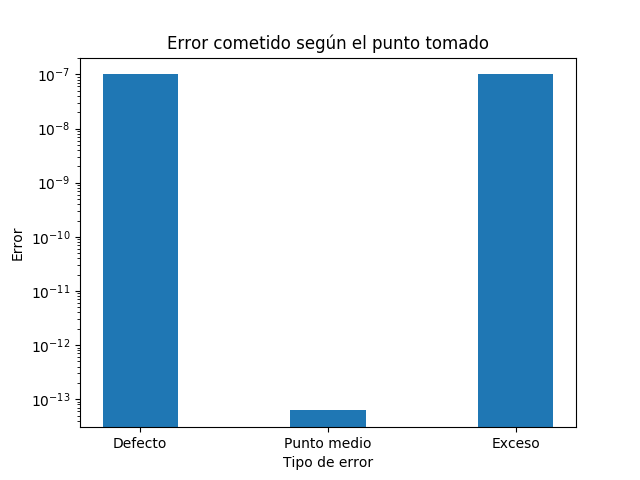
\includegraphics[scale=0.6]{img/error-puntos}
  \caption{Error cometido en la estimación según el punto donde se mide la integral, en escala
  logarítmica.}
  \label{fig:error}
\end{figure}

Como se puede ver en la figura \ref{fig:error}, el error por defecto y por exceso es casi el
mismo mientras que error en el punto medio es el menor de los tres. Este resultado es
completamente lógico, ya que al tomar el punto izquierdo se sobreestima el valor de la integral
mientras que al tomar el derecho se subestima. Al tomar el punto medio se equilibra el error que
se comete tanto por la derecha como por la izquierda, haciendo por tanto que la medida sea más
precisa.

\section{Estimación del número de intervalos}

Una vez que hemos determinado dónde medir el valor de la integral, vamos a ver cuántos intervalos
debemos utilizar. Vamos a probar algunos valores y veremos cómo va evolucionando el error
a medida que se incrementa el número de intervalos. Adicionalmente, vamos a medir también cuánto
tarda el cómputo para ir controlando que no nos excedamos de un límite de 10 segundos.

El número de intervalos que se han probado han sido $100000$, $1000000$, $10000000$, $100000000$,
$1000000000$ y $2000000000$, y los resultados obtenidos son los siguientes:

\begin{figure}[H]
  \centering
  \begin{minipage}{.5\textwidth}
    \centering
    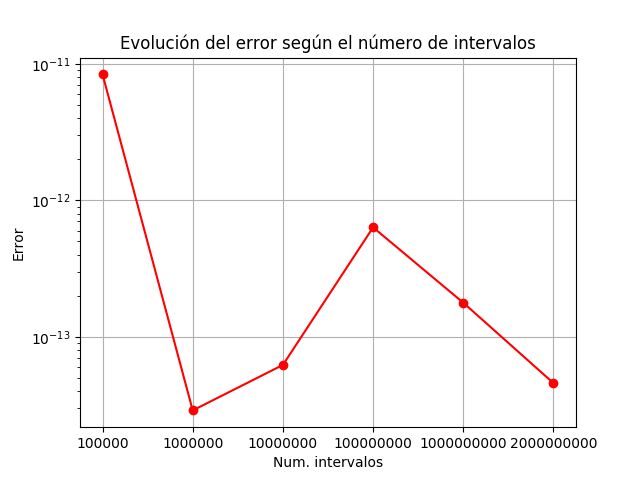
\includegraphics[scale=0.45]{img/evo-error}
  \end{minipage}%
  \begin{minipage}{.5\textwidth}
    \centering
    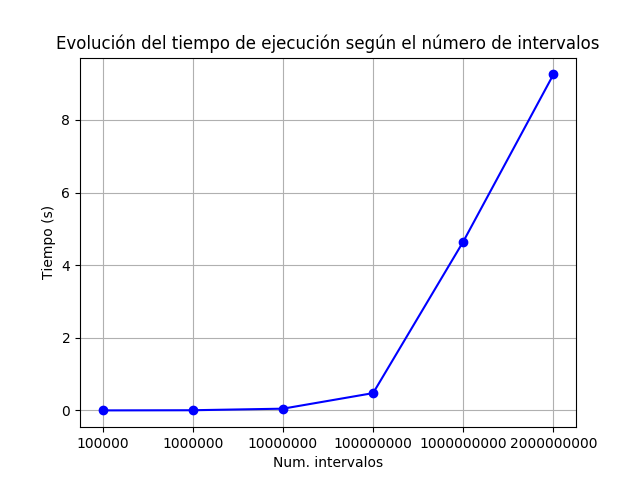
\includegraphics[scale=0.45]{img/evo-tiempo}
  \end{minipage}
  \caption{Evolución del error y del tiempo de ejecución según el número de intervalos.}
  \label{fig:intervalos}
\end{figure}

Tal y como podemos ver en la figura \ref{fig:intervalos}, el error tiene un comportamiento
irregular a medida que va aumentando el número de intervalos. Empieza bajando, pero al llegar
a los $1000000$ de intervalos comienza a crecer de nuevo. A partir de los $100000000$ de
intervalos empieza a decrecer de nuevo, y parece que sigue esa tendencia hasta el final.

El tiempo de ejecución, por otra parte, tiene un comportamiento más regular y estable.
A medida que se van aumentando el número de intervalos, el tiempo de ejecución va aumentando,
aunque en todo momento se mantiene por debajo de los 10 segundos.

Para elegir el mejor intervalo nos hemos fijado tanto en el tiempo de ejecución como en el
error obtenido. En este caso hemos elegido que se utilicen \textbf{$1000000000$ intervalos de
cálculo}, ya que con menos el tiempo de ejecución es muy pequeño y no merecería la pena
paralelizar, y con más, el tiempo se acerca demasiado al límite de 10 segundos que hemos impuesto.
Por tanto, se ha escogido la opción que presenta un equilibrio entre el tiempo de ejecución (algo
grande pero no en exceso) y el error obtenido (un error de aproximadamente $10^{-13}$ está
bastante bien).

\section{Paralelización del algoritmo}

Una vez que hemos determinado el punto en el que calcular la integral y cuántos intervalos
utilizar, vamos a paralelizar el algoritmo partiendo de la versión secuencial de este. Vamos
a ejecutarlo luego para 1, 2, 3 y 4 procesos y vamos a obtener los tiempos de inicialización,
cálculo y recepción de resultados en cada caso. Vamos a repetir cada ejecución tres veces y
obtendremos un tiempo medio junto con su desviación típica.

\subsection{Versión paralela del algoritmo}

La versión paralela del algoritmo secuencial utilizando \texttt{MPI} se puede ver a continuación:

\begin{lstlisting}
#include <stdio.h>
#include <stdlib.h>
#include <math.h>
#include <omp.h>
#include "mpi.h"

#define PI 3.141592653589793238462643

int main(int argc, char * argv[]) {
    double width, pi, sum, x;
    int intervals, i, myid, numprocs;
    double t, t_ini, t_comp, t_reduce;
    
    intervals = atoi(argv[1]);
    width = 1.0 / intervals;

    t = omp_get_wtime();

    MPI_Init(&argc, &argv);
    MPI_Comm_size(MPI_COMM_WORLD, &numprocs);
    MPI_Comm_rank(MPI_COMM_WORLD, &myid);
    
    if (myid == 0)
    {
        t_ini = omp_get_wtime() - t;
        t = omp_get_wtime();
    }    
    
    // Initialize sum
    sum = 0.0;
    
    // Do computation
    for (i = myid; i < intervals; i += numprocs)
    {
        x = (i + 0.5) * width;
        sum += 4.0 / (1.0 + x * x);
    }
    
    sum *= width;

    if (myid == 0)
    {
        t_comp = omp_get_wtime() - t;
        t = omp_get_wtime();
    } 
    
    // Reduce all values into pi
    MPI_Reduce(&sum, &pi, 1, MPI_DOUBLE, MPI_SUM, 0, MPI_COMM_WORLD);

    if (myid == 0)
    {
        t_reduce = omp_get_wtime() - t;
    } 

    MPI_Finalize();

    if (myid == 0)
    {
        printf("Number of intervals: %d\n", intervals);
        printf("PI is %0.24f\n", PI);
        printf("Estimation of PI is %0.24f\n", pi);
        printf("Error: %0.24f\n", fabs(PI - pi));
        printf("Initialization time: %f seconds\n", t_ini);
        printf("Computation time: %f seconds\n", t_comp);
        printf("Reduce time: %f seconds\n", t_reduce);
    }
    
    return 0;
}
\end{lstlisting}

Lo primero que se hace es inicializar \texttt{MPI} (líneas 19-21), obteniendo el tamaño
del comunicador y el rango de cada proceso. Después se hacen los cálculos y en la línea
48 se produce la recepción de los resultados, agrupando las sumas parciales en la variable de
salida \texttt{pi}. En la línea 55 se finaliza la sección paralela llamando a
\texttt{MPI\_Finalize()}. Una vez que se acaba, se muestran los resultados obtenidos y los
tiempos medidos.

\subsection{Tiempos obtenidos}

Una vez compilado el código anterior, se ha ejecutado siguiendo las especificaciones
anteriormente dadas. En la siguiente tabla se pueden ver los tiempos que se han obtenido:

\begin{table}[H]
\centering
\resizebox{\textwidth}{!}{%
\begin{tabular}{c|c|c|c|c|c|c|}
\cline{2-7}
 & \textbf{Núm. procesos} & \textbf{Tiempo 1 (s)} & \textbf{Tiempo 2 (s)} & \textbf{Tiempo 3 (s)} & \textbf{Media} & \textbf{Desviación} \\ \hline
\multicolumn{1}{|c|}{\multirow{4}{*}{\textbf{\begin{tabular}[c]{@{}c@{}}Tiempo\\ de\\ inicialización\end{tabular}}}} & 1 & 0.010941 & 0.009968 & 0.010388 & 0.01043233 & 0.00039846 \\ \cline{2-7} 
\multicolumn{1}{|c|}{} & 2 & 0.012234 & 0.011471 & 0.011520 & 0.01174167 & 0.00034871 \\ \cline{2-7} 
\multicolumn{1}{|c|}{} & 3 & 0.011469 & 0.012901 & 0.011492 & 0.011954 & 0.0006697 \\ \cline{2-7} 
\multicolumn{1}{|c|}{} & 4 & 0.014823 & 0.047699 & 0.023243 & 0.02858833 & 0.01394363 \\ \hline
\multicolumn{1}{|c|}{\multirow{4}{*}{\textbf{\begin{tabular}[c]{@{}c@{}}Tiempo\\ de\\ cómputo\end{tabular}}}} & 1 & 4.130078 & 4.128992 & 4.129614 & 4.12956133 & 0.00044492 \\ \cline{2-7} 
\multicolumn{1}{|c|}{} & 2 & 2.065498 & 2.065162 & 2.067519 & 2.06605967 & 0.00104098 \\ \cline{2-7} 
\multicolumn{1}{|c|}{} & 3 & 1.418354 & 1.418547 & 1.418820 & 1.41857367 & 0.00019118 \\ \cline{2-7} 
\multicolumn{1}{|c|}{} & 4 & 1.096716 & 1.146678 & 1.097349 & 1.113581 & 0.02340454 \\ \hline
\multicolumn{1}{|c|}{\multirow{4}{*}{\textbf{\begin{tabular}[c]{@{}c@{}}Tiempo\\ de\\ recepción\end{tabular}}}} & 1 & 0.000004 & 0.000006 & 0.000007 & \num{5.66666667e-06} & \num{1.24721913e-06} \\ \cline{2-7} 
\multicolumn{1}{|c|}{} & 2 & 0.000107 & 0.000122 & 0.000133 & \num{1.20666667e-04} & \num{1.06562449e-05} \\ \cline{2-7} 
\multicolumn{1}{|c|}{} & 3 & 0.000122 & 0.000134 & 0.000026 & \num{9.40000000e-05} & \num{4.83321839e-05} \\ \cline{2-7} 
\multicolumn{1}{|c|}{} & 4 & 0.000287 & 0.000030 & 0.000027 & \num{1.14666667e-04} & \num{1.21864223e-04} \\ \hline
\end{tabular}%
}
\caption{Resultados de cada ejecución junto con sus valores medios y desviación típica.}
\label{tab:my-table}
\end{table}

Según los resultados obtenidos, vemos que el tiempo de inicialización es, en general, más o
menos igual en todos los casos, salvo en el caso en el que se utilizan 4 procesos, donde los
tiempos individuales y el medio son algo superiores. Vemos también que en la mayoría de casos
hay poca variabilidad en los tiempos ya que la desviación típica es pequeña, menos en el caso
de 4 procesos, donde existe algo más de variabilidad y la desviación es algo mayor. Esta variación
podría deberse a que, al estar en una subred de máquinas interconectadas, en algún momento alguna
de las máquinas podría haber tenido una mayor carga, lo cuál se podría haber traducido en que se
tardase más en preparar el entorno de ejecución. A pesar de todo esto, los tiempos de
inicialización son, en general, pequeños, y representan una parte pequeña de todo el tiempo de
ejecución. Estos tiempos son tan pequeños porque estamos trabajando con muy pocos procesos (4 a lo
sumo). En caso de tener que crear más procesos sí que se hubiese podido notar algo más el tiempo
de inicialización, pero en casos tan pequeños es casi despreciable. Esta evolución se puede
ver mejor en la siguiente figura:

\begin{figure}[H]
  \centering
  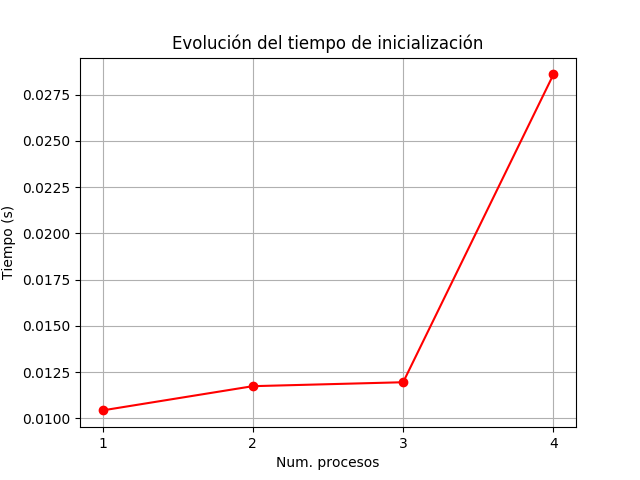
\includegraphics[scale=0.48]{img/evo-ini}
  \caption{Evolución del tiempo de inicialización.}
  \label{fig:ini}
\end{figure}

Si ahora analizamos el tiempo de cómputo, vemos que los tiempos obtenidos son bastante estables
en general, ya que las desviaciones típicas son bastante pequeñas, y por tanto, no hay mucha
variabilidad en los resultados. Si analizamos los tiempos medios, vemos que existe una clara
tendencia a que vayan decreciendo a medida que se van aumentando el número de procesos. Este
comportamiento es el esperado, ya que al tener más procesos, menos iteraciones del bucle va a
tener que realizar cada uno de ellos, con lo cuál el tiempo de ejecución será menor. El descenso
del tiempo de cómputo es muy pronunciado cuando se pasa de un proceso a dos. No obstante, cuando
se siguen aumentando el número de procesos el tiempo de cómputo no desciende tan bruscamente, si
no que lo hace de forma más suave. Este comportamiento puede verse en la siguiente figura:

\begin{figure}[H]
  \centering
  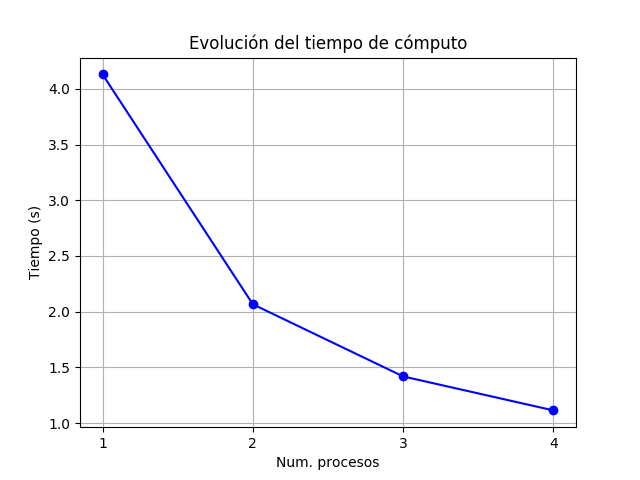
\includegraphics[scale=0.5]{img/evo-comp}
  \caption{Evolución del tiempo de cómputo en función del número de procesos.}
  \label{fig:comp}
\end{figure}

Como podemos ver, el ratio con el que desciende el tiempo de cómputo a medida que se van
aumentando el número de procesos parece que se va suavizando. Muy posiblemente, si probásemos
con más procesos, podríamos llegar a observar cómo el tiempo de cómputo se estanca y no mejora.

Por último, si observamos el tiempo de recepción de resultados, vemos que en el caso de un solo
proceso es casi despreciable, ya que al haber solo un proceso, no hay que esperar a que ninguno
otro se sincronice con este para recibir los datos. En los casos en los que hay más de un proceso
vemos que el tiempo de recepción no sigue un patrón claro ya que no existe una tendencia
a crecer o a decrecer tal y como pasaba con el tiempo de cómputo. Observamos también que existe
cierta variabilidad en los tiempos obtenidos ya que la desviación típica tiene un valor bastante
grande aunque estemos tratando con tiempos muy pequeños. La variabilidad puede deberse a que
algún proceso es algo más lento alguna de las veces, con lo cuál los demás lo tienen que esperar
para poder mandar los valores que han calculado (recordemos que \texttt{MPI\_Reduce()} es
bloqueante).

El comportamiento anteriormente mencionado del tiempo de recepción se puede ver a continuación:

\begin{figure}[H]
  \centering
  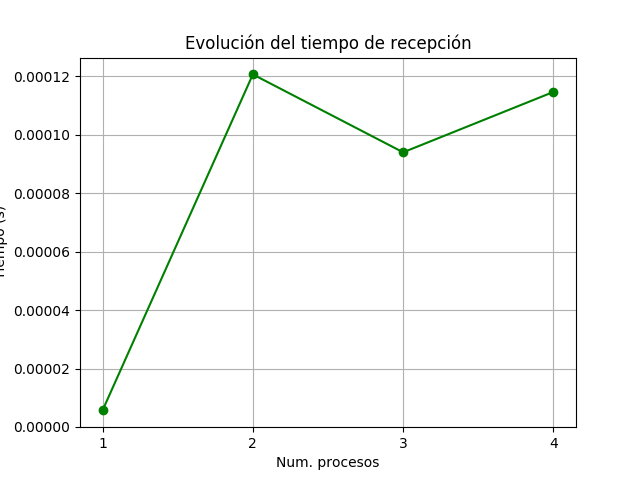
\includegraphics[scale=0.5]{img/evo-recep}
  \caption{Evolución del tiempo de recepción de resultados en función del número de procesos.}
  \label{fig:recep}
\end{figure}

Si observamos todos los tiempos medios de forma conjunta, nos encontramos ante lo siguiente:

\begin{figure}[H]
  \centering
  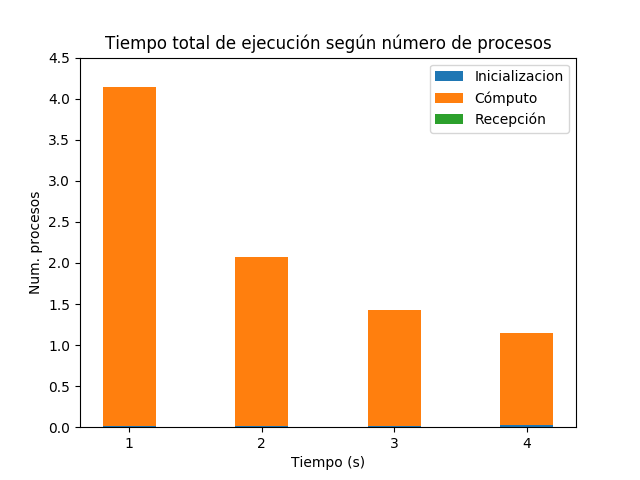
\includegraphics[scale=0.5]{img/evo-conjunta}
  \caption{Tiempos medios de inicialización, cómputo y recepción de forma conjunta para cada
   número de procesos.}
  \label{fig:recep}
\end{figure}

Vemos que en líneas generales la mayor parte del tiempo total de ejecución está en la parte de
cómputo. Los tiempos de recepción son casi despreciables, tanto que incluso no se ven muy bien.
Los tiempos de inicialización también son casi despreciables, aunque en el caso en el que se
utilizan 4 procesos sí que se nota algo más. Si tenemos en cuenta lo que hemos explicado
anteriormente, puede que al ir incrementando el número de procesos el tiempo de cómputo
llegue a estancarse en algún punto, mientras que el de inicialización posiblemente vaya
a ir subiendo a medida que se utilicen más procesos. Por tanto, es importante hacer un estudio
del tiempo de ejecución a medida que se van incrementando el número de procesos para determinar
cuál es el número ideal de estos.

\section{Ganancia obtenida}

Una vez que hemos estudiado los tiempos que hemos obtenido al paralelizar el código, vamos
a estudiar qué ganancia hemos obtenido en cada caso. A continuación se ofrece una tabla
con las ganancias, junto con una gráfica que muestra la evolución de esta en función del
número de procesos:

\begin{table}[H]
\centering
\begin{tabular}{|c|c|}
\hline
\textbf{Num. procesos} & \textbf{Ganancia} \\ \hline
1 & 1 \\ \hline
2 & 1.99876189 \\ \hline
3 & 2.91106583 \\ \hline
4 & 3.70836188 \\ \hline
\end{tabular}
\caption{Ganancia en velocidad en función del número de procesos.}
\label{tab:my-table2}
\end{table}

\begin{figure}[H]
  \centering
  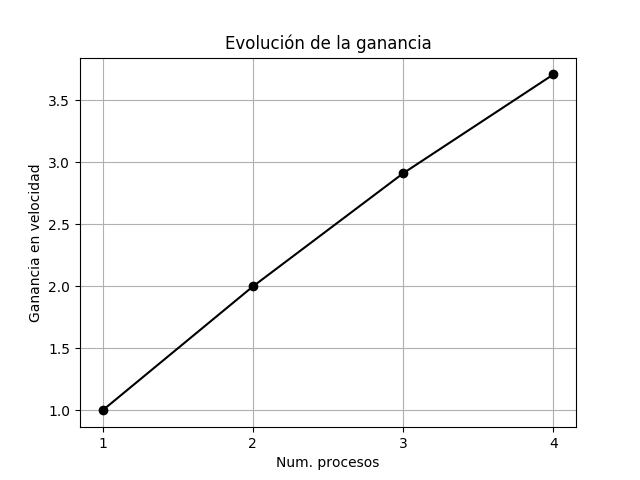
\includegraphics[scale=0.5]{img/ganancia}
  \caption{Evolución de la ganancia en velocidad según el número de procesos.}
  \label{fig:ganancia}
\end{figure}

Según podemos ver, la ganancia tiene un valor que se aproxima al número de procesos que
se estén utilizando, aunque se queda algo por debajo. Vemos que a medida que aumenta el
número de procesos, la ganancia se va quedando cada vez más por debajo de dicho número.
Por tanto, aunque en un principio parezca que la ganancia es lineal al número de procesos,
en realidad la ganancia sería algo inferior a la lineal, ya que de seguir utilizando más
procesos seguramente se llegaría a que en algún momento la ganancia está bastante por debajo
del número de procesos utilizado. Por tanto, llegaría un momento en el que añadir más procesos
no aportaría ninguna mejora; es más, podría incluso llegar a empeorar los tiempos si se tienen en
cuenta tiempos de creación y de comunicación.

De esta forma, podemos decir que la ganancia está acotada a un valor máximo, aunque tendríamos que
o bien seguir probando con más procesos o bien hacer un estudio teórico para determinar cuál es
ese valor.

\section{Conclusiones}

En esta práctica hemos partido de un algoritmo secuencial para el cálculo de $\pi$ y al estudiarlo
hemos visto que puede ser paralelizado, ya que el bucle del cálculo puede ser fácilmente
paralelizado.

Hemos implementado una versión paralela de este y, tras hacer algunas pruebas y un estudio, hemos
visto que el tiempo de cálculo se va reduciendo a medida que se utilizan más procesos. Sin
embargo, al haber estudiado la ganancia al paralelizar el algoritmo, hemos visto que esta está
acotada, ya que la ganancia no es lineal. Por tanto, llegaría un punto en el que no obtendríamos
una mejora significativa del tiempo de cómputo a pesar de estar utilizando muchos procesos.

De esta forma, debemos escoger cuidadosamente el número de procesos que queremos utilizar debido a
que en caso de escoger demasiados podríamos tener consecuencias no deseadas, como por ejemplo un
\textit{overhead} por comunicación o por la creación de los procesos.


\end{document}

